% Uncomment this to make slides with overlays:
%\documentclass[slides]{beamer}

% Uncomment these (but comment the above \documentclass line) to make handouts:
\documentclass[handout]{beamer}

% Uncomment these to have more than one slide per page
\usepackage{pgfpages}
\pgfpagesuselayout{2 on 1}[border shrink=5mm]
\pgfpageslogicalpageoptions{1}{border code=\pgfusepath{stroke}}
\pgfpageslogicalpageoptions{2}{border code=\pgfusepath{stroke}}

\usepackage[]{graphicx, color, hyperref}

\mode<presentation>
{
	%\usetheme[secheader]{Boadilla}
	%\usecolortheme[rgb={.835, .102,.169}]{structure}  
	\usetheme[width= 0cm]{Goettingen}
	%\setbeamercovered{transparent}
}
\setbeamertemplate{navigation symbols}{}
\setbeamertemplate{footline}[frame number]

\definecolor{blue2}{rgb}{0.278,0.278,0.729} 
\newcommand{\blue}[1]{\textcolor{blue2}{#1}}
\newcommand{\white}[1]{\textcolor{white}{#1}}
\newcommand{\red}[1]{\textcolor{red}{#1}}
\newcommand{\xbar}{\overline{x}}
\newcommand{\ybar}{\overline{y}}
\newcommand{\phat}{\widehat{p}}
\newcommand{\prob}{\mbox{Pr}}
\newcommand{\E}{\mathbb{E}}
\newcommand{\Var}{\mbox{Var}}
\newcommand{\cp}{\oplus}
\newcommand{\cm}{\circleddash}

\title{Lecture 15: Hypothesis Testing Part II}
\author{Chapter 4.3}
\date{}


\begin{document}
%------------------------------------------------------------------------------
\begin{frame}
\titlepage
\end{frame}
%------------------------------------------------------------------------------


%-------------------------------------------------------------------------------
\begin{frame}
\frametitle{Previously... Statistical Hypothesis Testing}

A \blue{hypothesis test} is a method for using sample data to decide between two competing hypotheses about the population parameter:
\pause \begin{itemize}
\item A \blue{null hypothesis $H_0$}.\\
i.e. the \blue{status quo} that is initially assumed to be true, but will be tested. 
\item An \blue{alternative hypothesis $H_A$}. i.e. the \blue{challenger}.
\end{itemize}

\vspace{0.25cm}

\pause There are two potential outcomes of a hypothesis test.  Either we
\begin{itemize}
\item reject $H_0$  
\item fail to reject $H_0$
\end{itemize}
\end{frame}
%-------------------------------------------------------------------------------


%-------------------------------------------------------------------------------
\begin{frame}
\frametitle{Previously... Decision Errors}
Hypothesis tests will get things right sometimes and wrong sometimes:
\pause \begin{center}
  \begin{tabular}{cc|cc}
     \multicolumn{2}{c}{}  & \multicolumn{2}{c}{\textbf{Test conclusion}} \\ 
     &  & do not reject $H_0$ & reject $H_0$ in favor of $H_A$ \\ 
\hline
    \textbf{Truth} & $H_0$ true & OK & \blue{Type I Error} \\ 
     & $H_A$ true & \blue{Type II Error} & OK \\ 
    \hline
  \end{tabular}
\end{center}

\pause\vspace{0.25cm}

Two kinds of errors:
\begin{itemize}
\item \blue{Type I Error}: a false positive (test result)
\item \blue{Type II Error}: a false negative (test result)
\end{itemize}

\end{frame}
%-------------------------------------------------------------------------------


%-------------------------------------------------------------------------------
\begin{frame}
\frametitle{Type I Errors:  US Criminal Justice System}
Defendants must be proven ``guilty beyond a reasonable doubt'': in theory they would rather let a guilty person go free, than put an innocent person in jail.  

\pause\vskip 0.25cm

\begin{itemize}
\item $H_0$: the defendant is innocent
\item $H_A$: the defendant is guilty
\end{itemize}
\pause thus ``rejecting $H_0$'' is a guilty verdict $\Rightarrow$ putting them in jail

\vskip 0.25cm

\pause In this case:
\begin{itemize}
\item Type I error is putting an innocent person in jail\\
(considered worse)
\item Type II error is letting a guilty person go free.  
\end{itemize}
\end{frame}
%-------------------------------------------------------------------------------


%-------------------------------------------------------------------------------
\begin{frame}
\frametitle{Type II Errors: Airport Screening}
An example of where Type II errors are more serious:  \blue{airport screening}. 

\pause \begin{eqnarray*}
H_0: && \mbox{passenger X does not have a weapon}\\
H_A: && \mbox{passenger X has a weapon}
\end{eqnarray*}
\pause Failing to reject $H_0$ when $H_A$ is true is not ``patting down'' passenger X when they have a weapon.
\vskip 0.25cm
\pause Hence the long lines at airport security.  
\end{frame}
%-------------------------------------------------------------------------------


%------------------------------------------------------------------------------
\begin{frame}[fragile]
\frametitle{Goals for Today}

\begin{itemize}
\item Define significance level
\item Tie-in p-Values with sampling distributions
\item Example
\end{itemize}

\end{frame}
%------------------------------------------------------------------------------


%-------------------------------------------------------------------------------
\begin{frame}
\frametitle{Significance Level}
%Hypothesis testing is built around rejecting or failing to reject the null hypothesis.\\
%\pause i.e. we do not reject $H_0$ unless we have \blue{strong evidence}.
%
%\pause \vspace{0.5cm}
%
%As a rule of thumb, when $H_0$ is true, we do not want to incorrectly reject $H_0$ more than 5\% of the time.\\
%i.e. $\alpha = 0.05 = 5\%$ is the \blue{significance level}.  
%
%\pause \vspace{0.5cm}
%
%With 95\% confidence intervals from earlier, we expect it to miss the true population parameter 5\% of the time.  This corresponds to $\alpha=0.05$.   
\end{frame}
%-------------------------------------------------------------------------------


%-------------------------------------------------------------------------------
\begin{frame}
\frametitle{Thought experiment: p-Values}
Say you flip a coin you think is fair 1000 times.  Say you observe
\begin{itemize}
\pause \item 501 heads? Do you think the coin is biased?
\pause \item 525 heads? Do you think the coin is biased?
\pause \item 900 heads? Do you think the coin is biased?
\end{itemize}

\end{frame}
%-------------------------------------------------------------------------------


%-------------------------------------------------------------------------------
\begin{frame}
\frametitle{Thought experiment: p-Values}

Intuitively, a \blue{p-value} quantifies how \blue{extreme} an observation is given the null hypothesis.  
  
\vskip 0.25cm

\pause The smaller the p-value, the more \blue{extreme} the observation, where the meaning of extreme depends on the context.  

\vskip 0.25cm

\pause Note the p-value is different than the population proportion $p$ (bad historical choice).

\end{frame}
%-------------------------------------------------------------------------------


%-------------------------------------------------------------------------------
\begin{frame}
\frametitle{p-Values}
%Definition:  The \blue{p-value} or \blue{observed significance level} is the probability of observing a test statistic as extreme or more extreme (in favor of the alternative) as the one observed, assuming $H_0$ is true.
%
%\vspace{0.5cm}
%
%\pause It is \blue{NOT} the probability of $H_0$ being true.  This is the most common misinterpretation of the $p$-value.

\end{frame}
%-------------------------------------------------------------------------------


%# Binomial
%p.hat <- rep(0,1000)
%for(i in 1:10000) {
%  samp <- sample(c(0,1), 1000, replace=TRUE)
%  p.hat[i] <- mean(samp)
%}
%
%pdf("./7.1 Hypothesis Testing/hist1.pdf", width=6, height=6)
%hist(p.hat, xlab="proportion", main="Fair Coin Histogram")
%dev.off()
%
%pdf("./7.1 Hypothesis Testing/hist2.pdf", width=6, height=6)
%hist(p.hat, xlab="proportion", main="Observed 501 Heads")
%abline(v=501/1000, col="red", lwd=2)
%dev.off()
%
%pdf("./7.1 Hypothesis Testing/hist3.pdf", width=6, height=6)
%hist(p.hat, xlab="proportion", main="Observed 525 Heads")
%abline(v=525/1000, col="red", lwd=2)
%dev.off()
%
%pdf("./7.1 Hypothesis Testing/hist4.pdf", width=10, height=6)
%hist(p.hat, xlim=c(440/1000,900/1000), xlab="proportion", main="Observed 900 Heads")
%abline(v=900/1000, col="red", lwd=2)
%dev.off()


%-------------------------------------------------------------------------------
\begin{frame}
\frametitle{Recall our Coin Example}
%You have a coin that test for fairness with $n=1000$ flips.  Set $p_0 = 0.5$ and define a ``success'' as getting heads.  \pause i.e.
%\begin{eqnarray*}
%&& H_0: p = p_0 \mbox{ i.e. coin is fair}\\
%vs && H_A: p \neq p_0
%\end{eqnarray*}
%
%\begin{itemize}
%\pause \item The point estimate $\widehat{p}$ of $p$ is $\frac{\mbox{\# of successes}}{\mbox{\# of trials}}$.
%\pause \item Since it is based on a sample, $\widehat{p}$ has a sampling distribution
%\pause \item The standard error is $\sqrt{\frac{p(1-p)}{n}}$ (Chapter 6).
%\pause \item Furthermore, since conditions hold, the sampling distribution is Normal (CLT)
%\end{itemize}
\end{frame}
%-------------------------------------------------------------------------------


%-------------------------------------------------------------------------------
\begin{frame}
\frametitle{Sampling Distribution of $\widehat{p}$}
\blue{Under $H_0$ that the coin is fair} i.e. $p=p_0=0.5$, the sampling distribution of $\widehat{p}$ when $n=1000$ is:

\begin{center}
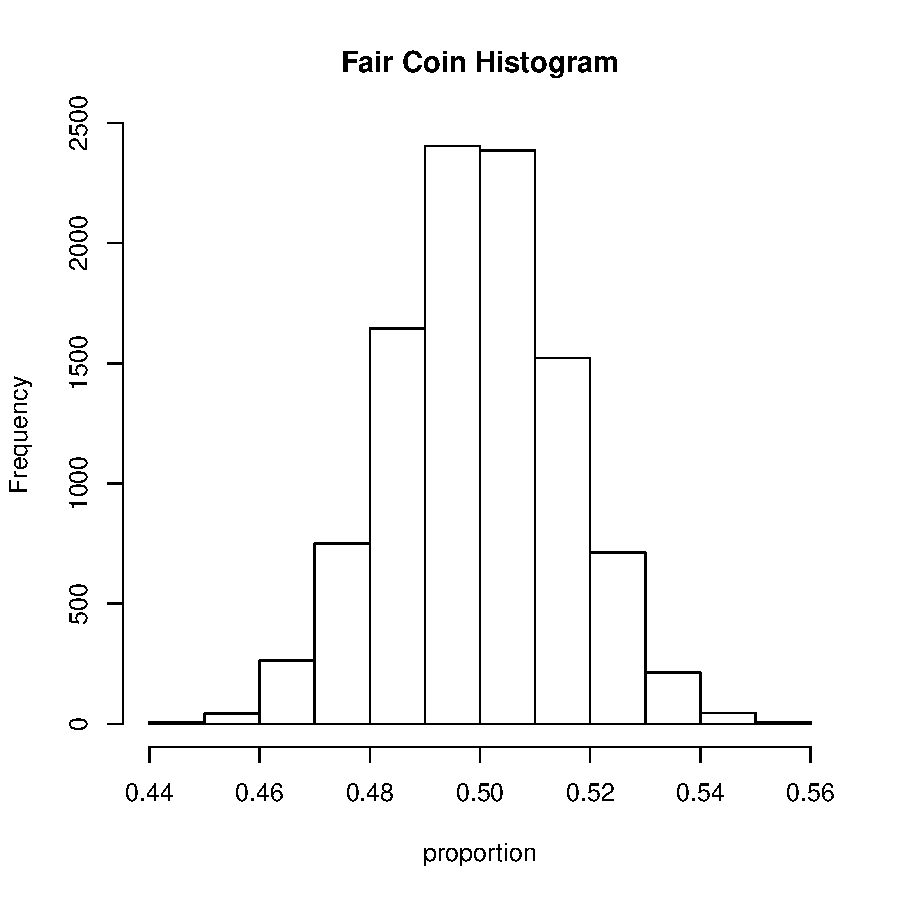
\includegraphics[width=0.6\textwidth]{figure/hist1}
\end{center}
\end{frame}
%-------------------------------------------------------------------------------


%%-------------------------------------------------------------------------------
%\begin{frame}
%\frametitle{Intuition Behind p-Values}
%Intuitively, a \blue{p-value} quantifies how \blue{extreme} an observation is given the null hypothesis.  
%
%\vskip 0.5cm
%
%The smaller the p-value, the more \blue{extreme} the observation, where the meaning of extreme depends on the context.  
%
%\end{frame}
%%-------------------------------------------------------------------------------
%%-------------------------------------------------------------------------------
%\begin{frame}
%\frametitle{Intuition Behind p-Values}
%You flip another coin \blue{you know is fair} (i.e. $p=0.5$) 1000 times and compute the proportion of heads.
%
%\vspace{0.25cm}
%
%Do this a bunch of times and plot a histogram.  
%
%\vspace{0.25cm}
%
%Compare this histogram to the results of your friend's coin.  
%
%\end{frame}
%%-------------------------------------------------------------------------------


%-------------------------------------------------------------------------------
\begin{frame}
\frametitle{Say we observe...}
\begin{center}
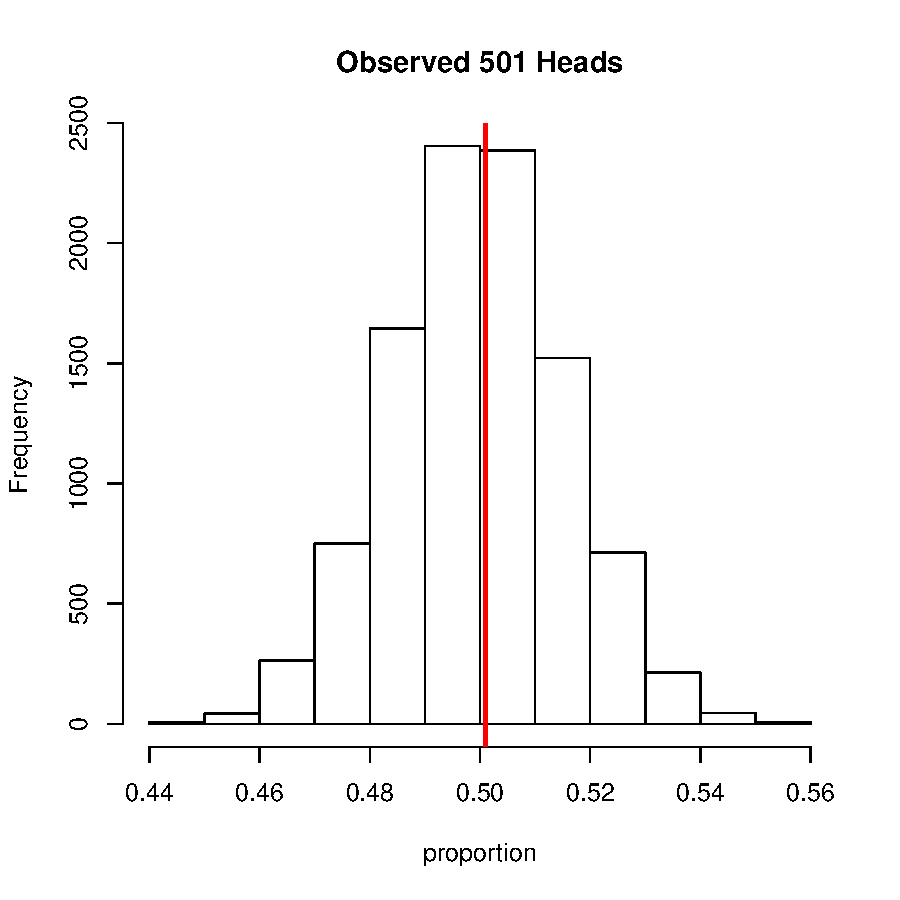
\includegraphics[width=0.6\textwidth]{figure/hist2}
\end{center}
\end{frame}
%-------------------------------------------------------------------------------


%-------------------------------------------------------------------------------
\begin{frame}
\frametitle{Say we observe...}
\begin{center}
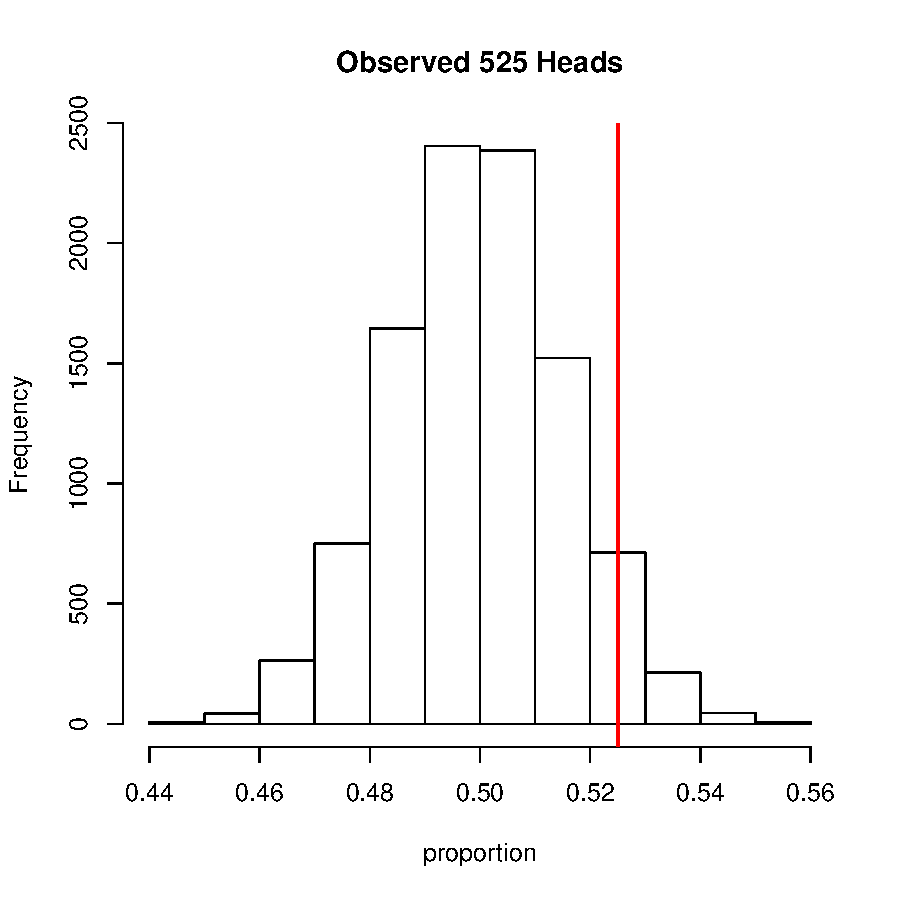
\includegraphics[width=0.6\textwidth]{figure/hist3}
\end{center}
\end{frame}
%-------------------------------------------------------------------------------


%-------------------------------------------------------------------------------
\begin{frame}
\frametitle{Say we observe...}
\begin{center}
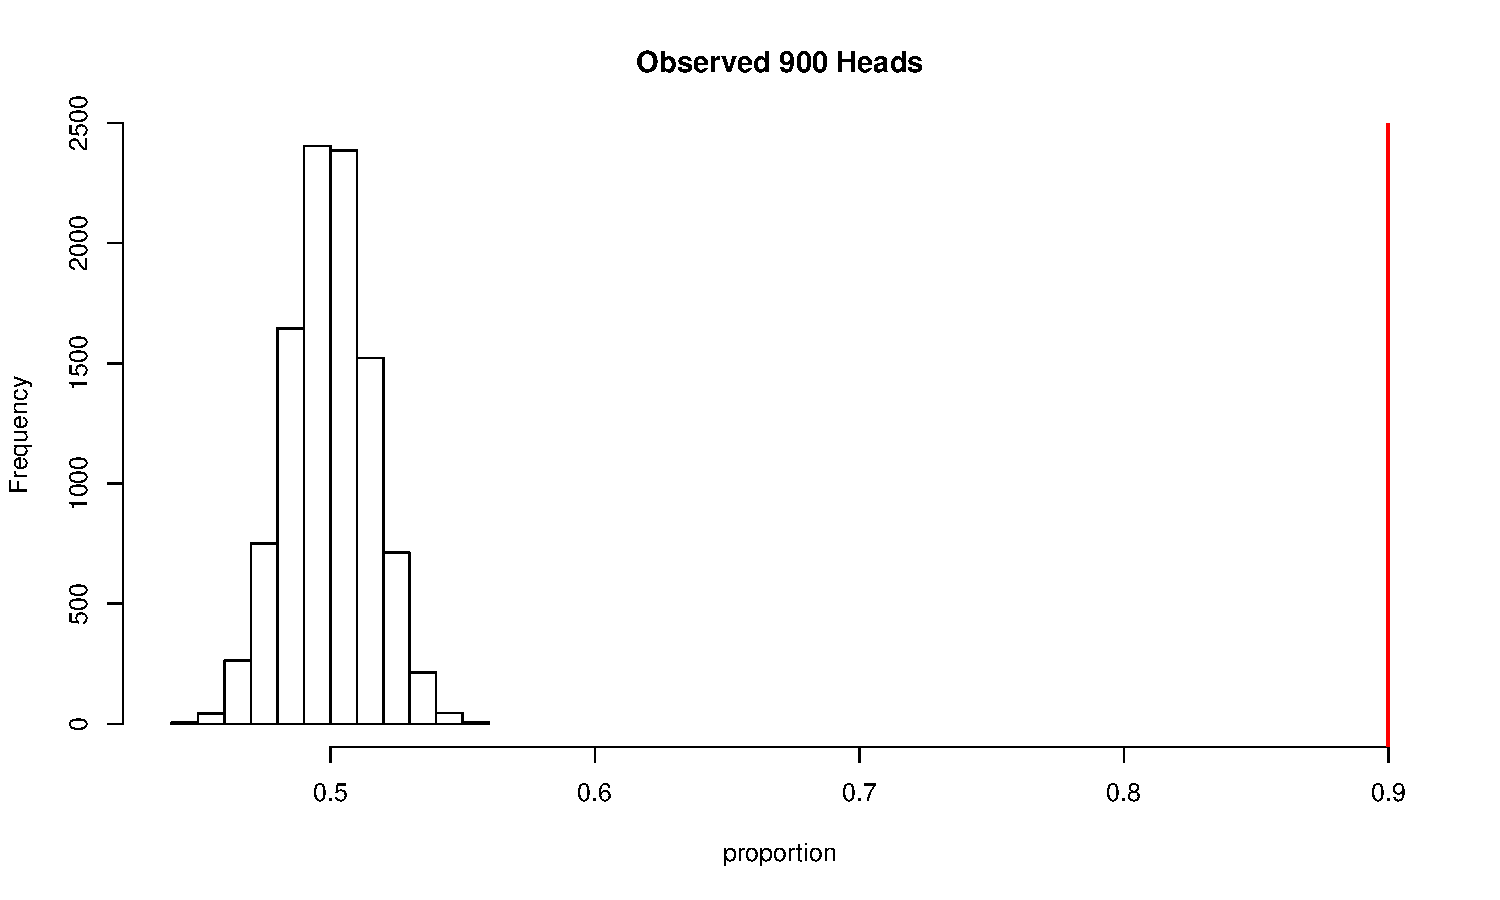
\includegraphics[width=\textwidth]{figure/hist4}
\end{center}
\end{frame}
%-------------------------------------------------------------------------------


%%-------------------------------------------------------------------------------
%\begin{frame}
%\frametitle{p-Value Definition}
%The \blue{p-value} or \blue{\textit{observed} significance level} is the probability of observing a test statistic as extreme or more extreme (in favor of the alternative) as the one observed, assuming $H_0$ is true.
%
%\vspace{0.5cm}
%
%It is \blue{NOT, NOT, NOT} the probability of $H_0$ being true.  This is the most common misinterpretation of the $p$-value.
%
%\end{frame}
%%-------------------------------------------------------------------------------


%%-------------------------------------------------------------------------------
%\begin{frame}
%\frametitle{Coin Example Hypothesis Testing}
%The \blue{null value} $0.5$ is the prob of a heads assuming the null hypothesis is true.  i.e. the coin is fair.  
%
%\vspace{0.5cm}
%
%Say we suspected that the prob of getting a head was greater than 0.5.  We have the following competing \blue{one-sided} hypotheses
%\begin{itemize}
%\item $H_0: p = 0.5$
%\item $H_A: p > 0.5$
%\end{itemize}
%
%\vspace{0.5cm}
%
%The p-value is the probability, in the case, of getting a value to the \blue{right} of the red line.  
%
%
%\end{frame}
%%-------------------------------------------------------------------------------


%-------------------------------------------------------------------------------
\begin{frame}
\frametitle{Example about Sleep Habits}
A poll found that college students sleep about 7 hours a night.  Researchers suspect that Reedies sleep more.   They want to investigate this claim at a pre-specified $\alpha=0.05$ level.  \pause They sample $n=110$ Reedies and find that $\xbar = 7.42$ and $s=1.75$ and the histogram looks like:

\begin{center}
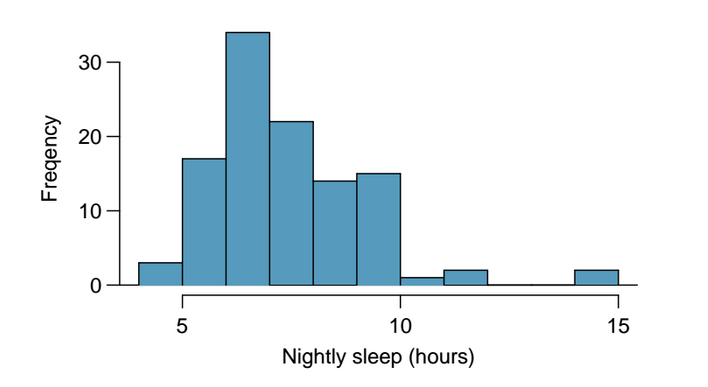
\includegraphics[width=0.6\textwidth]{figure/sleep.png}
\end{center}


%\vspace{0.5cm}

%Let $\mu = $ \blue{true population mean} \# of hours Reedies sleep a night.  Then $\mu_0=7$ and: 
%\begin{itemize}
%\item $H_0: \mu = \mu_0= 7$
%\item $H_A: \mu > 7$
%\end{itemize}
%
%\vspace{0.5cm}
% hence $z=\frac{7.42 - 7}{\frac{1.75}{\sqrt{110}}} = 2.47$.

\end{frame}
%-------------------------------------------------------------------------------


%-------------------------------------------------------------------------------
\begin{frame}
\frametitle{Example about Sleep Habits}


\end{frame}
%-------------------------------------------------------------------------------







%-------------------------------------------------------------------------------
\begin{frame}
\frametitle{Example about Sleep Habits}
In our case, since $H_A: \mu > 7$, \blue{more extreme} means \blue{to the right} of $z=2.47$.  

\vspace{0.5cm}

Hence, the p-value is 0.007:

\begin{center}
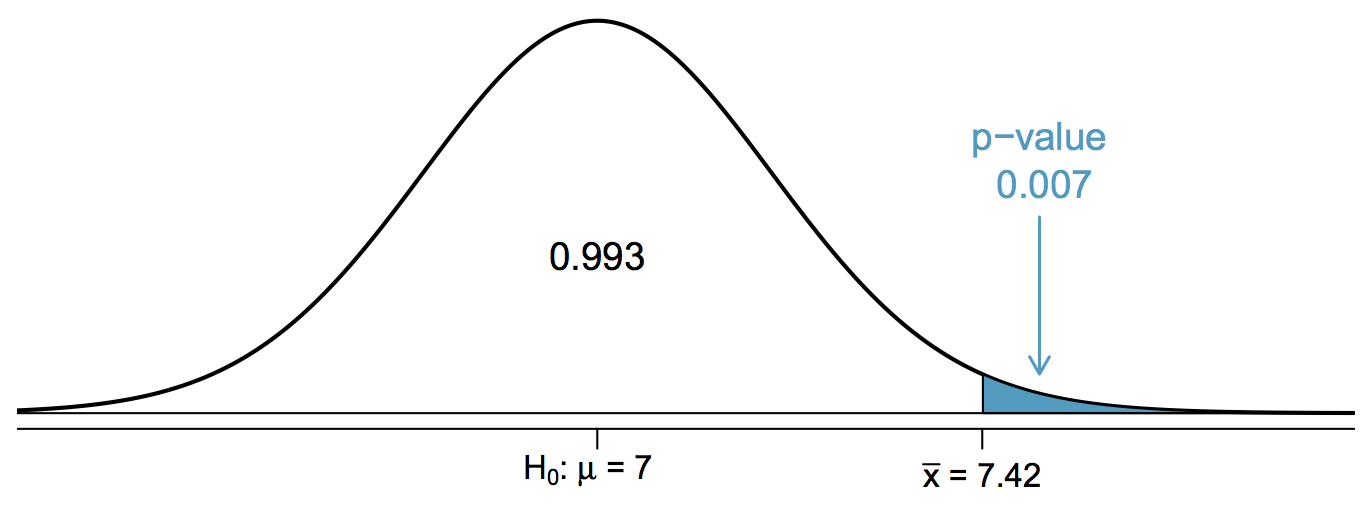
\includegraphics[width=\textwidth]{figure/pvalue.png}
\end{center}

\end{frame}
%-------------------------------------------------------------------------------


%-------------------------------------------------------------------------------
\begin{frame}
\frametitle{Example about Sleep Habits}
Since the p-value $0.007 < 0.05=\alpha$, the \blue{pre-specified} significance level, it has a high degree of \blue{extremeness}, and thus we \blue{reject $H_0$}.

\vspace{0.5cm}

\pause\blue{Interpretation}: we reject (at the $\alpha=0.05$ significance level) the hypothesis that the average \# of hours of Reedies sleep is 7, in favor of the hypothesis that sleep more.    

\end{frame}
%-------------------------------------------------------------------------------


%-------------------------------------------------------------------------------
\begin{frame}
\frametitle{Example about Sleep Habits}
\blue{Correct interpretation of the p-value}:  If the null hypothesis is true ($\mu=7$), the probability of observing a sample mean $\xbar=7.42$ or greater is 0.007.  

\vspace{0.5cm}

\pause \blue{Incorrect interpretation of the p-value}:  The probability that the null hypothesis ($\mu=7$) is true is 0.007.  

\end{frame}
%-------------------------------------------------------------------------------



%%-------------------------------------------------------------------------------
%\begin{frame}
%\frametitle{Example about Sleep Habits}
%
%Researchers find that $\xbar = 7.42$ and $s=1.75$.  Before we proceed, we check the 3 conditions to use the Normal model:
%\begin{enumerate}
%\pause \item Independence: $n=110 \leq$ 10\% of 1,453 (Reed enrollment)
%\pause \item $n \geq 30$
%\pause \item The distribution of the $n=110$ observations (Figure 4.14) is not too skewed.
%\end{enumerate}
%
%\end{frame}
%%-------------------------------------------------------------------------------


%%-------------------------------------------------------------------------------
%\begin{frame}
%\frametitle{Example about Sleep Habits}
%
%\blue{Question to keep in mind}:  What if the null hypothesis were true (i.e. the null value $\mu_0=7$)?
%
%\pause \vspace{0.5cm}
%
%How likely are we to observe $\xbar=7.42$ or something more extreme in favor of the alternative, i.e. greater?  Use the $z$-score of $\xbar$. 
%
%\pause \vspace{0.5cm}
%
%Remember in general
%\[
%z = \frac{x-\mu}{\sigma}
%\]
%\pause So in our case for $\xbar$
%\[
%z = \frac{\xbar - \mu \mbox{ when $H_0$ is true }}{SE} = \frac{\xbar - \mu_0}{SE} = \frac{7.42 - 7}{\frac{1.75}{\sqrt{110}}} = 2.47
%\]
%
%\end{frame}
%%-------------------------------------------------------------------------------


%%-------------------------------------------------------------------------------
%\begin{frame}
%\frametitle{Example about Sleep Habits}
%
%If the null hypothesis were true, then $\xbar$ would have come from the following nearly normal distribution.  The $p$-Value is 0.007 since:
%
%\begin{center}
%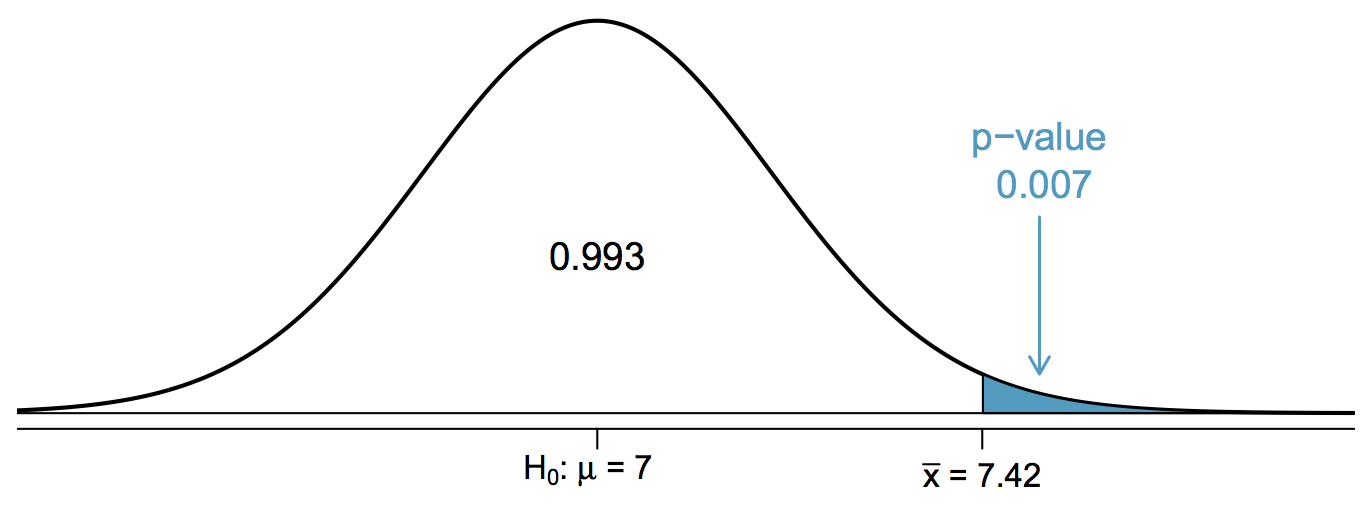
\includegraphics[width=\textwidth]{figure/pvalue.png}
%\end{center}
%
%\end{frame}
%%-------------------------------------------------------------------------------


%%-------------------------------------------------------------------------------
%\begin{frame}
%\frametitle{Example about Sleep Habits}
%
%\blue{Correct interpretation}:  If $H_0$ is true, the probability of observing a sample mean $\xbar=7.42$ or greater is only 0.007.  
%
%\pause \vspace{0.5cm}
%The p-value quantifies how strongly the data favor $H_A$ over $H_0$.  A small $p$-value corresponds to sufficient evidence to reject $H_0$ in favor of $H_A$.  
%
%
%\pause \vspace{0.5cm}
%Final decision.  Since we set $\alpha=0.05$ \blue{beforehand} and the p-value $0.007 < 0.05 = \alpha$, we reject the null hypothesis.  i.e. based on evidence, we believe Reedies sleep more than 7 hours a night.  
%
%\end{frame}
%%-------------------------------------------------------------------------------


%%-------------------------------------------------------------------------------
%\begin{frame}
%\frametitle{Recall Example about Reedie Sleep Habits}
%
%Let $\mu$ be the true \blue{population mean} \# of hours Reedies sleep a night.  Then:
%\begin{itemize}
%\item $H_0: \mu = 7$
%\item $H_A: \mu > 7$
%\end{itemize}
%
%\vspace{0.5cm}
%
%Researchers find that $\xbar = 7.42$ and $s=1.75$.
%
%\vspace{0.5cm}
%
%7.42 is bigger than the \blue{null value} 7, suggesting $H_A$ is true.  Is it bigger enough however?
%
%\end{frame}
%%-------------------------------------------------------------------------------


%%-------------------------------------------------------------------------------
%\begin{frame}
%\frametitle{Example:  Exercise 4.28 on Page 177 on Sleep}
%
%We need to account for the variability of $\xbar$.
%
%\vspace{0.5cm}
%
%Standardize $\xbar$ (find the z-score) assuming $H_0$ is true: $\mu=7$.  i.e. that
%\begin{itemize}
%\item $\xbar$ has mean equal to the null value 7
%\item $\xbar$ has standard deviation $SE=\frac{1.75}{\sqrt{110}} = 0.167$ (the standard error)
%\end{itemize}
%
%\end{frame}
%%-------------------------------------------------------------------------------


%%-------------------------------------------------------------------------------
%\begin{frame}
%\frametitle{Example:  Exercise 4.28 on Page 177 on Sleep}
%We must we check the 3 conditions
%\begin{enumerate}
%\item Independence: the sample size $n=110$ is less than 10\% of 1,453 (Reed enrollment).
%\item The sample size is greater than $30$.
%\item The distribution of the $n=110$ observations (Figure 4.14) is not too skewed.
%\end{enumerate}
%
%We can assume the normal model holds!
%
%\end{frame}
%%-------------------------------------------------------------------------------




%%-------------------------------------------------------------------------------
%\begin{frame}
%\frametitle{Example:  Exercise 4.28 on Page 177 on Sleep}
%Remember in general, we standardize a value as follows:
%\[
%z = \frac{x-\mu}{\sigma}
%\]
%So in our case for $\xbar$
%\[
%z = \frac{\xbar - \mbox{null value}}{SE} = \frac{7.42 - 7}{\frac{1.75}{\sqrt{110}}} = 2.47
%\]
%
%\end{frame}
%%-------------------------------------------------------------------------------


%
%
% Laying this out now makes the procedure too formulaic
%
%
%%-------------------------------------------------------------------------------
%\begin{frame}
%\frametitle{In General:  Hypothesis Testing Procedure}\label{ht}
%\begin{enumerate}
%\pause\item Construct your hypothesis testing framework:
%\begin{itemize}
%\item Define $H_0$, $H_A$ and if applicable a null value.
%\item Set your significance level $\alpha$
%\end{itemize}
%\pause\item Verify that the conditions hold
%\pause\item Compute your \blue{test statistic}
%\pause\item Compute the p-value
%\begin{itemize}
%\item Identify the appropriate distribution to compare the test statistic to
%\item Depending on $H_A$, determine what constitutes being \blue{more extreme} and compute the p-value using the appropriate probability table.
%\end{itemize}
%\pause\item If the p-value is $< \alpha$, reject $H_0$.  Otherwise do not.
%\end{enumerate}
%
%\end{frame}
%%-------------------------------------------------------------------------------


%%-------------------------------------------------------------------------------
%\begin{frame}
%\frametitle{In Reedie Sleep Example}
%\begin{enumerate}
%\pause\item Construct your hypothesis testing framework:
%\begin{itemize}
%\item Define $H_0$, $H_A$ and if applicable a null value.
%\item Set your significance level $\alpha$
%\end{itemize}
%\pause\item Verify that the conditions hold
%\pause\item Compute your \blue{test statistic}: \textcolor{red}{the z-score of $\xbar=7.42$}
%\pause\item Compute the p-value
%\begin{itemize}
%\item Identify the appropriate distribution to compare the test statistic to:  \textcolor{red}{normal distribution}
%\item Depending on $H_A$, determine what constitutes being \blue{more extreme} and compute the p-value using the appropriate probability table: \textcolor{red}{z-table on page 409}
%\end{itemize}
%\pause\item If the p-value is $<\alpha$, reject $H_0$.  Otherwise do not.
%\end{enumerate}
%
%\end{frame}
%%-------------------------------------------------------------------------------


%------------------------------------------------------------------------------
\begin{frame}[fragile]
\frametitle{Next Time}

\begin{itemize}
\item How big a sample size to I need? i.e. power calculations
\item Statistical vs practical significance
\end{itemize}

\end{frame}
%------------------------------------------------------------------------------


\end{document}










